\chapter{Background}

\section{Monoids}

We begin our background with a review on monoids.
Monoids are pervasive in category theory, and we will see themes and elements from the basic monoid construction in practically every following definition.
This comes from a simple fact: functions form monoids.

The monoid is one of the most basic and rudimentary algebraic structures that can be endowed on a set.
It consists of an associative binary operator and an identity element.

More formally, given a set $X$, a monoid is a tuple $(X,\cdot, e)$ where $\cdot:X\times X\rightarrow X$ is the aforementioned binary operator satisfying
\begin{equation}
	(x\cdot y)\cdot z = x\cdot(y\cdot z)
\end{equation}
for all $x,y,z\in X$,
and $e\in X$ is an identity element satisfying
\begin{equation}
	e\cdot x = x\cdot e = x
\end{equation}
for all $x\in X$.

In the spirit of moving towards category theory in which we shy away from working with elements and reason with functions, we can equivalently write the identity element as a function from the singleton set $e: \singletonset \rightarrow X$.
If we rename the binary operator to a variable name such as $m$ so that we think of it more like a function in the traditional sense, then the above associativity and identity relations can be rewritten as the following commuting diagrams:
\todo[inline]{Make commuting diagrams with m and e, using function pairings (m,e) etc for the products}

A basic example is the natural numbers with addition: $(\naturals, +, 0)$ forms a monoid.
Notice that multiplication also works, and $(\naturals, \times, 1)$ forms a monoid structure as well.
The $0$ and the $1$ elements interact in such a way as to form a rig.

A more important example is functions. The space of endofunctions $X^X := \{f:X\rightarrow X\}$ forms a monoid with function composition $(X^X, \circ, \id)$, where $\id$ is the identity function that does nothing.

Another important example is sets themselves, with Cartesian product and the singleton set.
If we denote the class\footnote{Later, category} of sets as $\Set$, then $(\Set, \times, \singletonset)$ form a monoid.
Rather, it's not quite strictly a monoid, because we have a loosening of the associativity and identity conditions.
Notice how the set $X\times(Y\times Z)$ is equal to the set of points $\{(x,(y,z)):x\in X, y\in Y, z\in Z\}$, whereas
$(X\times Y)\times Z = \{((x,y),z):x\in X, y\in Y, z\in Z\}$.
They're not quite equal to each other.
They are, however, naturally isomorphic, meaning that for each set $X$ $Y$ and $Z$, there is an associator isomorphism $\alpha_{X,Y,Z}: (X\times Y)\times Z \rightarrow X\times (Y\times Z)$ which maps tuples of elements as $\alpha : ((x,y),z) \mapsto (x,(y,z))$.
Being an isomorphism, this map is invertible.

Similarly, notice how $\singletonset \times X = \{(\cdot, x):x\in X\}$ and $X\times \singletonset = \{(x,\cdot):x\in X\}$, which both are not identical to $X$.
However, for each $X$ there are unit isomorphisms $\eta_{l;X} : \singletonset \times X \rightarrow X$ with $\eta_{l;X} : (\cdot, x) \rightarrow x$ and $\eta_{r;X} : X \times \singletonset \rightarrow X$ with $\eta_{r;X} : (x,\cdot) \rightarrow x$ which absorb the singleton element.
These are also easily invertible.

We typically hand-wave all these details away in the math world, especially if we treat all nested tuples as automatically flattening and all singleton elements as automatically absorbing.
However, if we were to formalize Cartesian products in a programming language, then we would either need to specify this nested flattening or we would need to program in unit and associator isomorphisms and be extremely careful in applying them so that the types match correctly.

We should also note that as Cartesian products involve making pairs of elements, we can also make pairs of functions:
for $f : X\rightarrow Y$ and $g:A\rightarrow B$, we can form the function $(f,g) : X\times A \rightarrow Y\times B$ with $(f,g)((x,a)) = (f(x), g(a))$.
From now on, we will instead write this as $f\times g$, to relate it back to the Cartesian product.
This shows that the Cartesian product is actually bifunctorial, which makes $\Set$ a monoidal category.

\subsection{Symmetric monoids}

A monoid is symmetric if $x\cdot y = y\cdot x$.

In our above examples, notice that $(\naturals, +,0$ is indeed symmetric, as $a+b=b+a$, but $(X^X, \circ, \id)$ is not, because order matters in composition: $f\circ g \neq g\circ f$.

For $\Set$, we have a similar situation to above: it's not strictly symmetric, but for every $X$ and $Y$ there's a swap natural isomorphism $\sigma_{X,Y} : X\times Y \rightarrow Y\times X$ with $\sigma_{X,Y} : (x,y) \mapsto (y,x)$.

\section{Category Theory}

\subsection{Categories}

A category formally is a collection of objects and morphisms that follow a composition law \cite{context}. \todo{Expand on this. Should I give an actual definition of an abstract category? I probably should}

While this definition is very abstract, it is useful in describing a lot of things \todo{find a better word} in mathematics.
Some of the most useful categories for application are \emph{concrete} categories, which practically are categories whose objects spaces with some form of structure and morphisms are structure preserving mappings between them.


\missingfigure{Make a diagram to represent a few objects/morphisms in $\Set$.}
\missingfigure{Make a diagram to represent a few objects/morphisms in $\FinVect$. Make it look congruent to $\Set$.}

An example is shown in $\Set$ and $\FinVect$.
The category $\Set$ has sets as its objects, and its morphisms are functions.
The category $\FinVect$ has as its objects finite dimensional vector spaces over the real numbers as their bed of scalars, and its morphisms are linear transformations\footnote{These transformations can be represented by a matrix, but only if a basis is provided for both domain and codomain. We should not automatically assume a vector space has a canonical basis that's best for the job!}.
Note that $\FinVect$ is just a subcategory\footnote{I won't define it, but I hope it's not hard to imagine what a subcategory is. Closure under composition is the main requirement.} of $\Set$. This is talked about in more detail in books.\todo{Specify}

This view is different from a set theoretic approach to fields in mathematics.
For instance, the set theoretic approach to linear algebra would define a vector space as a set with a certain algebraic structure, and a linear transformation as a function preserving that structure in a certain way.
A categorical approach would instead define the category of vector spaces as a collection of objects (the vector spaces) and of morphisms\footnote{and of functors. more on that later}, and would specify how morphisms behave in composition.
This approach is described as "context rich and content poor"\todo{cite youtube video}
\todo[inline]{Finish this paragraph. Element poor, but we can get around that, and the language is unified to describe similar phenomena in different fields, blah blah blah}

\todo[inline]{Talk about functional programming}
\todo[inline]{Talk about how Markov categories are cats with markov kernels}

%\subsection{Functors}
%\subsubsection{Example Functors}
%\subsection{Monoidal Functors}
%\subsection{Natural Transformations}
%\subsection{Monads}
%\subsection{Kleisli Categories}

\section{Markov Categories}

Markov categories are categories in which the morphisms behave like stochastic kernels.
There are in fact Markov categories that have too restrictive of a structure to represent the probability we're interested in, but we can build a Markov category out of the kernels that we model problems with for computation.
When we formulate problems in terms of Markov categories, we can then revert to the language of category theory and abstract away the details of which computations the morphisms in a particular Markov category represent.

More specifically, a good way to think about a Markov category is that the objects represent classes of distributions\footnote{While most of the time objects are enumerated by the underlying statespace (or dimension for that matter), it's helpful to think of them as the collections of distributions themselves}, and the morphisms are mappings between them.

For example, the spaces and mappings discussed in Section \ref{the kalman filter kernels section} form the Markov category $\gausscat$.
Each object is $\gaussian X$, the collection of Gaussian distributions on the vector space $X$.
The morphisms are the kernels specified in Equations \ref{gaussian kernels}.

\subsection{Definition}

A Markov category is a symmetric monoidal category with comonoidal objects.
Practically, we should break this definition up into its components and axioms.

\subsubsection{A Markov category is a category}

A category is made out of objects and morphisms that go between them.
For our practial purposes our Markov categories will be concrete, meaning that the objects represent sample spaces and the morphisms represent mappings between them.
In literature, objects are typically given names that correspond to the underlying sample space such as $X$ and $Y$.
This is particularly appropriate for deterministic categories such as $\Set$, which is indeed a Markov category, but the categories we're interested in should represent transition kernels between classes of distributions.
Thus, for clarity, throughout this section we will think of objects with capital letters $X$, $Y$, etc.\ as sets, and the objects in our Markov category will be labeled as $\probfunc X$, $\probfunc Y$, etc.\ to emphasize that we are thinking of them as classes of distributions on the underlying sets.

Thus, a Markov category is composed of classes of distributions $\probfunc X$, $\probfunc Y$, etc.\ and transition kernels between them that look like $f:\probfunc X \rightarrow \probfunc Y$.

In our program, this means we will be creating two datatypes: one that constructs kernels, and one that \emph{parameterizes} the underlying spaces.
We do not need to make a datatype for the underlying space itself.
We will see why later.

For example, for $\gausscat$, we will make a datatype representing the kernels that look like Equation \ref{gaussian kernels}.
We will also need a datatype whose elements parameterize all the spaces $\gaussian X$, but we don't need a separate datatype for each $\gaussian X$ itself.
Since the underlying spaces $X$ are just relabelings of $\reals^n$, every class of Gaussian distributions can be uniquely labeled by the dimenision $n$ of its underlying space.
Thus, it is sufficient to parameterize the classes of Gaussian distributions by the natural numbers $\naturals$.

The basic axioms that must be satisfied are composition and identity:
for every $f:\probfunc X \rightarrow \probfunc Y$ and $g:\probfunc Y \rightarrow \probfunc Z$, there must be another kernel from $\probfunc X$ to $\probfunc Z$ that we denote $g\circ f$.

Composition must be associative, ie.
\begin{equation}
	(h\circ g)\circ f = h\circ (g\circ f)
\end{equation}
for all $f,g,h$ where their types line up.

In our program, this means that we must make a method for composing two kernels, and they must satisfy associativity.

Categories also have identity morphisms.
For every space $X$, there must be a "do nothing" kernel $\id_X : \probfunc X \rightarrow \probfunc X$ that satisfies
\begin{align}
	\id_X \circ f &= f\\
	g\circ \id_X &= g
\end{align}
for all $f:\probfunc W\rightarrow \probfunc X$ and $g:\probfunc X\rightarrow \probfunc Y$.

In our program, we must create a constructor method `id()` that takes in the parameter that represents $X$ and creates a respective identity function.
It may seem trivial and unnecessary to require such a constructor.
This kernel does afterall represent doing nothing.
However, its is extremely important as we will use it to build more complicated kernels.

\subsubsection{A Markov category is symmetric monoidal}

A symmetric monoidal category is a category in which the objects form a (not necessarily strict) symmetric monoid, much like the $\Set$ example in Section \ref{monoids}.

So in our Markov category, for every class of distributions $\probfunc X$ and $\probfunc Y$, there must be a class $\probfunc (X\times Y)$.
This corresponds to the class of distributions over the joint states.

Notice that the Cartesian product is placed inside the probability functor.
We could well have a category where where the monoidal structure gives objects $\probfunc X \times \probfunc Y$, but these are a bit too strict for our purposes.
In fact, $\Set$ itself is indeed a Markov category, with its monoidal structure being a direct Cartesian product.
However, there are further conditions on the universality of the Cartesian product that make $\Set$ just a bit too strict to form an interesting Markov category.
In particular, as will be discussed below, an element $z\in X\times Y$ can be reconstructed if we only know its projections $\pi_l(z) = x$ and $\pi_r(z) = y$.
We will get similar projection operators in our less-deterministic Markov category, which correspond to marginialization, but we cannot reconstruct a probability distribution from its marginals.
Therefore, to undercut the probability functor, in some cases we will need to introduce a zipping function $\laxator_{X,Y} : \probfunc X\times \probfunc Y\rightarrow \probfunc(X\times Y)$, also called a laxator, to refactor our data.
This may or may not be discussed more below. I haven't decided yet.

In monoidal categories, not only does 

\subsubsection{Objects in a Markov category are comonoids}

\subsection{Example: Set}
\subsection{Kleisli Categories}

\section{String Diagrams}

String diagrams are very similar to the signal flow diagrams or block diagrams found in control systems.
Others (\cite{baez2015control}, \cite{fong2016thesis}, \cite{fong2016dynamicalsystems}) have drawn the connections between string diagrams and various diagrams in systems engineering including block diagrams for dynamical systems.

There are often two interpretations in block diagrams:
In what I will call the temporal interpretation, the state of a diagram can be seen as changing over time, where the states are carried by the wires from block to block. The blocks represent state transformations, which are applied continuously to their inputs to generate changing outputs.
There may be blocks which carry their own internal state, such as integrators, that keep track of quantities over time to affect their output\todo{This sentence sucks.}

In what I'll call the signal flow interpretation, a time-varying signal is seen as a single entity, and the blocks represent signals in transformation space. This interpretation allows for a more functional analysis type approach to control design.

String diagrams look quite similar to block diagrams, but their interpretation is very different.
Blocks are still seen as transformations, but they then become the primary point of interest instead of the "signals" themselves.
The wires do not represent signals, but rather state spaces.
Whenever a wire splits, or disappears, or loops around, that becomes interpreted as a special transformation itself.
With this interpretation, a string diagram simply becomes a tool to draw out complicated compositions of transformations, or morphisms in a symmetric monoidal category.

\subsection{Explanation of String Diagrams}

\subsection{Translating String Diagrams into Kernel Compositions}
String diagrams allow us to write complicated equations with a single picture that can then be systematically translated back into equations for computation.
These pictures are often much clearer to interpret, and easier to memorize as they can be puzzle pieced together.
Interpreting them is straightforward: Take the example problem of finding the conditional of a kernel with respect to part of its output.
This problem statement carries with it the nuance of the complexity in finding conditionals, unlike the simple measure theoretic definition.

Given $f:A\rightarrow X\otimes Y$, find $f_X : X\otimes A \rightarrow Y$ such that the equation in Figure \ref{fig:conditional} holds.

\begin{figure}[htb]
	\centering
	\tikzfig{conditional}
	\caption{The string diagram equation for the definition of conditioning.}
	\label{tikz:conditional}
\end{figure}

\begin{figure}[htb]
	\centering
	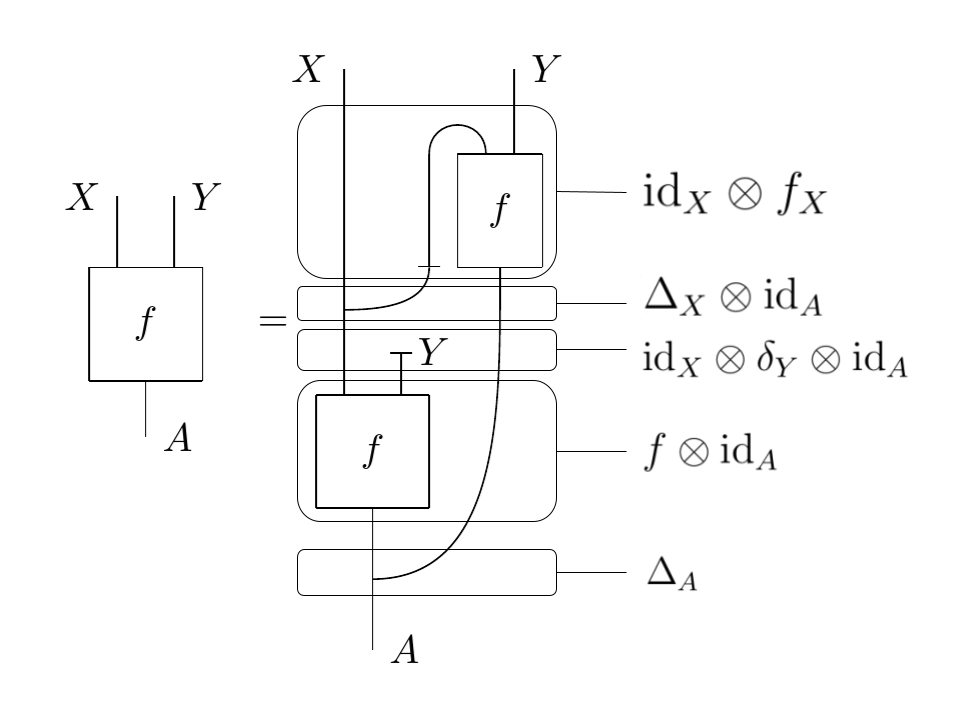
\includegraphics[width=0.8\textwidth]{conditional-compositions}
	\caption{The conditional equation is read like so. This corresponds to Equation \ref{eq:conditional-compositions}.}
	\label{fig:conditional-compositions}
\end{figure}

\begin{figure}[htb]
	\centering
	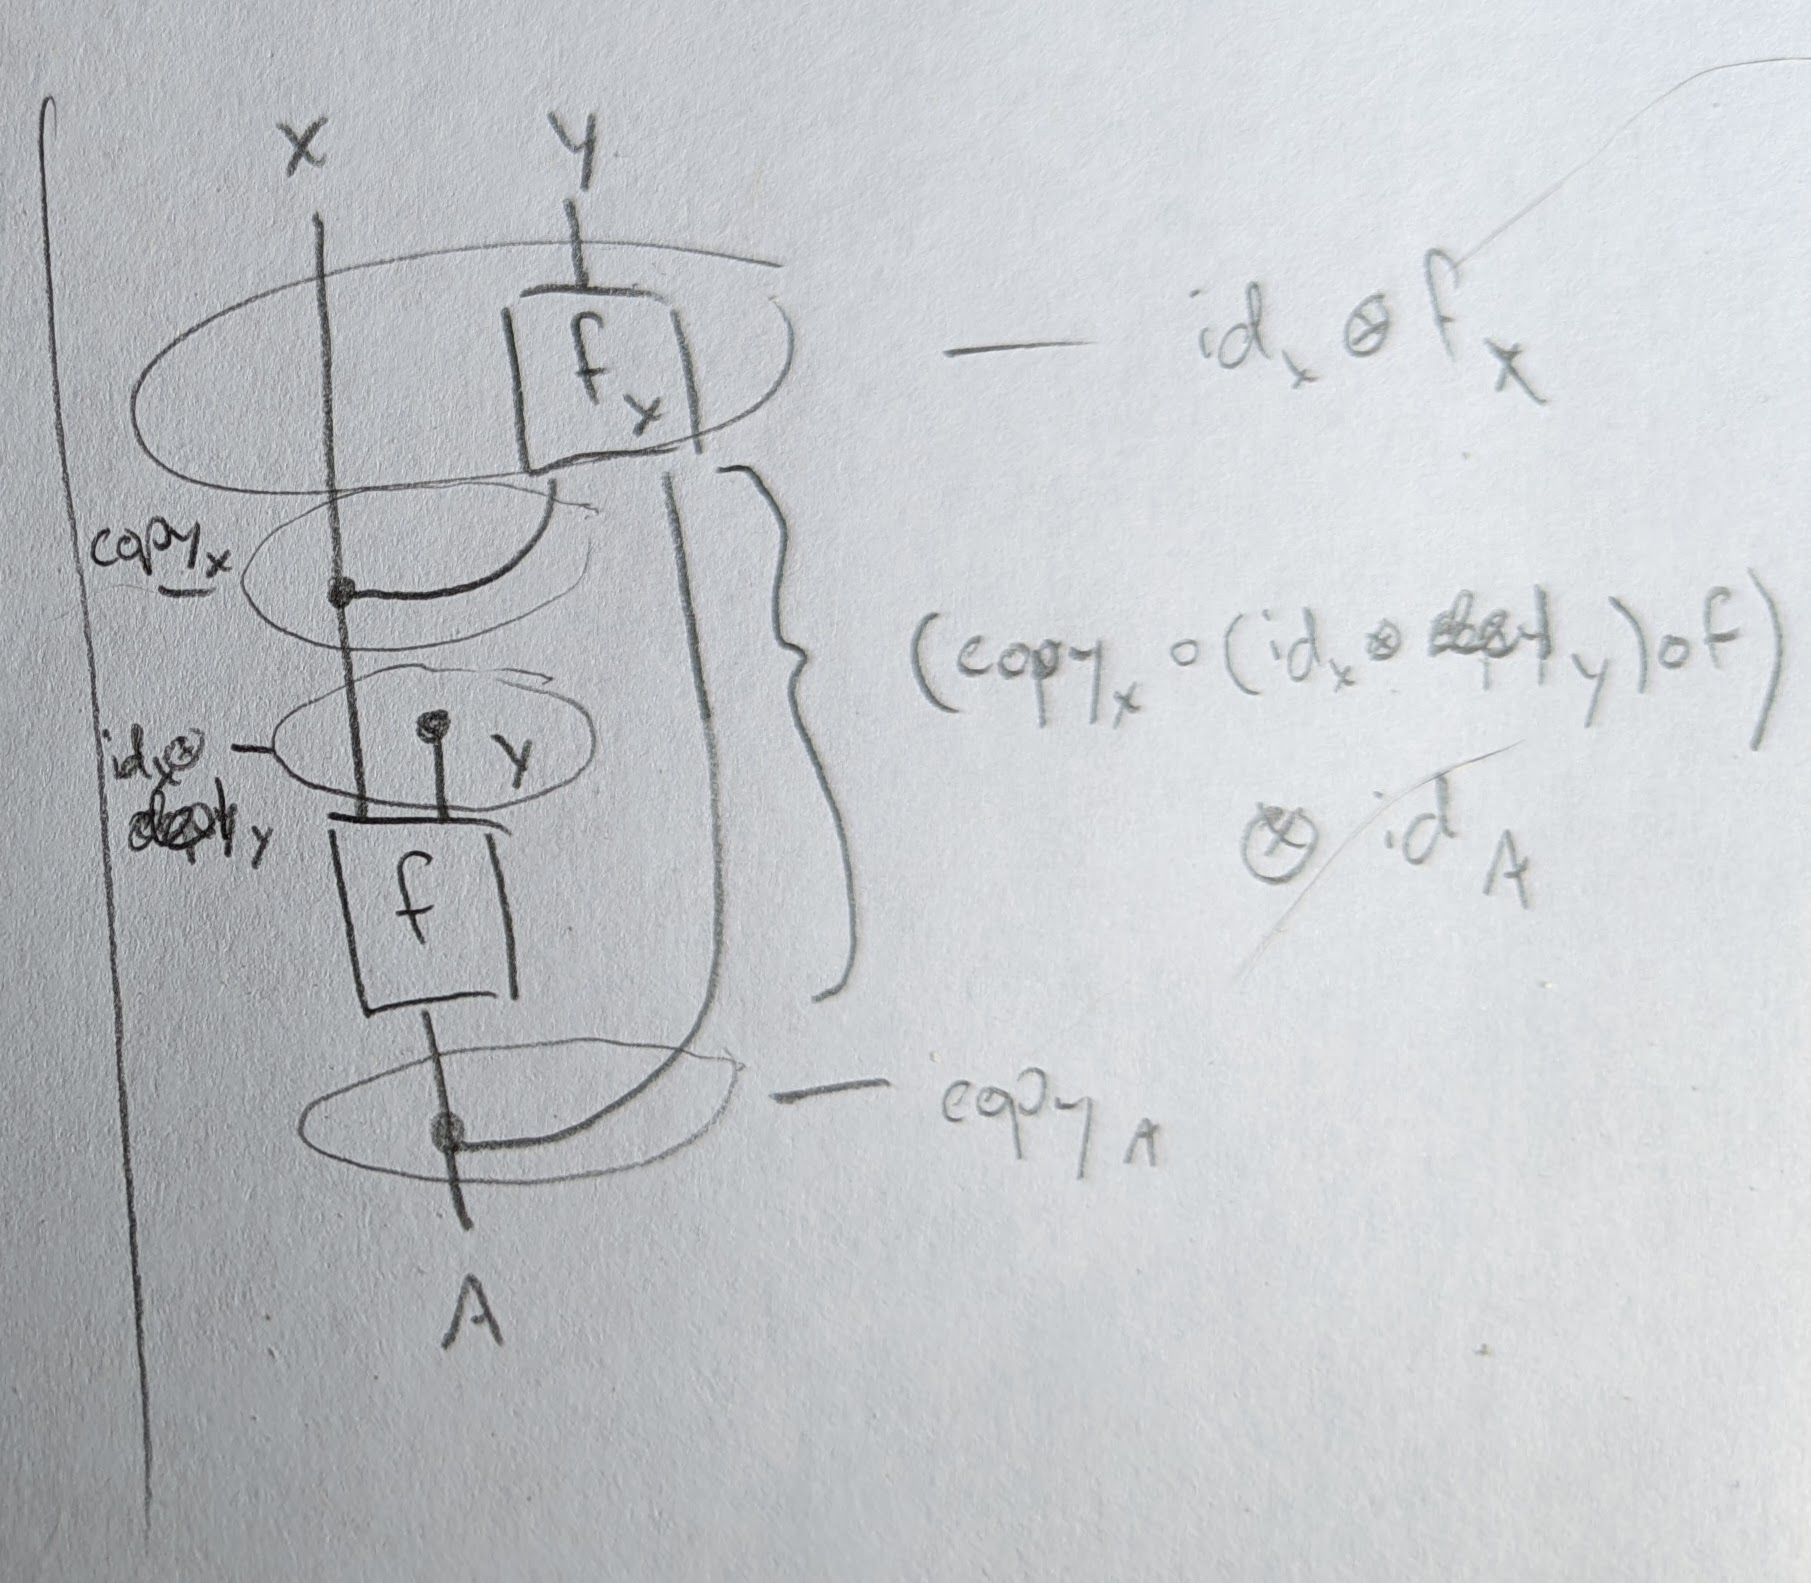
\includegraphics[width=0.5\textwidth]{conditional-parallel-compositions}
	\caption{The conditional equation can also be read this way. This corresponds to Equation \ref{eq:conditional-parallel-compositions}.}
	\label{fig:conditional-parallel-compositions}
\end{figure}

\begin{equation}
\label{eq:conditional-compositions}
f = (\id_X \otimes f_X) \circ (\comul_X \otimes \id_A)
\circ (\id_X \otimes \counit_Y \otimes \id_A) \circ (f \otimes \id_A) \circ \comul_A
\end{equation}

\begin{equation}
\label{eq:conditional-parallel-compositions}
f = (\id_x \otimes f_x) \circ \left[\left(\comul_x \circ (\id_x\otimes \counit_Y) \circ f\right) \otimes \id_A\right] \circ \comul_A
\end{equation}

** Explain notation. Every operator you are using in these equations should be explained and formally introduced. **

\section{Bar Notation}
\subsection{Explanation of Bar Notation}
\subsection{Translating Bar Notation into String Diagrams}

\chapter{Common Representations of Information Recast into the Language of Markov Categories}
\section{Discrete Probability}
\section{Gaussian Probability}
\section{Gaussian Mixtures: A Composition of Discrete and Gaussian Probability}

The framework in this section was developed with much help from Tobias Fritz in the Category theory Zulip channel \cite{zulip}

We now develop Gaussian mixtures in purely abstract terms.
First let's discuss Gaussian mixtures concretely.

A basic explanation of Gaussian mixtures is that a Gaussian mixture distribution is a convex combination of Gaussian distributions.
More formally, if we have $p_i: I\rightarrow X$, then a Gaussian mixture distribution can be defined as
\begin{equation}
    p = \sum_i w_i | p_i \rangle
\end{equation}
where every $w_i \geq 0$, and $\sum_i w_i = 1$.
Here we use the ket notation as in \cite{cho-jacobs}.
This can be interpreted as a point-wise summation on the PDFs of the Gaussians, or we can keep it as a formal sum ie.\ a sequence of pairs.

Notice that the collection of these convex combinations is precisely the finite distribution monad $\distributionmonad$ applied not to the space $X$, but seemingly to the collection of Gaussians $\gaussian X$.

\subsection{Distributive Laws}

A first approach would to be try distributive laws.
In essence, these allow you to compose monads.
This unfortunately will not work for Gaussian mixtures for several reasons, but this can still yield us new Markov categories by combining old ones.

Given two monads $(S,\mu^S, \eta^S)$ and $(T, \mu^T,\eta^T)$, a distributive law of $S$ over $T$ is a natural transformation
\begin{equation}
    l:TS\rightarrow ST
\end{equation}
satisfying certain conditions. \todo{Should I write these conditions? Probably if I want to prove the following.}

An important feature here is that we can compose the monads, at least in one direction as $ST$, to form a new monad.
In partcular, the join and unit NTs become
\begin{align}
    \mu^{ST} &: STST \xrightarrow{SlT} SSTT \xrightarrow{\mu^S \mu^T} ST\\
    \eta^{ST} &: 1\xrightarrow{\eta^S\eta^T}ST
\end{align}

Remember that Markov categories arise from symmetric monoidal affine monads on other Markov categories.
Thus, if $T,\ S\in C$ are symmetric monoidal affine monads, with laxators $\laxator^T$ and $\laxator^S$ respectively, then $ST$ will\todo{prove this} become symmetric monoidal affine with
\begin{equation}
    \laxator^{ST}_{X,Y} : STX \otimes STY \xrightarrow{\laxator^S_{TX,TY}}
    S(TX\otimes TY) \xrightarrow{S\laxator^T_{X,Y}} ST(X\otimes Y)
\end{equation}

Thus, we can now compose two probability monads to make a third.
Unfortunately, however, this will not help us with Gaussian mixtures.
For one, $\gaussian$ is not an endofunctor, and $\gausscat$ is not a Kleisli category.
We simply abuse the notation for convenience.
And even if we were to try to treat $\gaussian$ as an endofunctor, the composition wouldn't make sense.
The distributive law $l$ requires the functor compositions to go both ways. 
It would make sense to construct $\distributionmonad\gaussian X$ as a convex combination of Gaussian distributions on $X$, but not so much for $\gaussian \distributionmonad X$, a Gaussian distribution of convex combinations of $X$'s.

Still, we should push this further. Let's try to come up with conditioning on $ST$.
\todo[inline]{Dr. Bakolas this is where I need help}

\subsection{Markov functor}

What if we have a Markov functor to another Markov category, and then apply a monoidal monad to its image?
This should work, but it still won't give us what we want I don't think.

\subsection{Monads Applied to Hom Sets}

One way that will work with Gaussian mixtures is to use a hom set construction.

If we consider a Markov category $C$, then the space of distributions on $X\in C$ is equivalent to the hom set $C(1,X)$.
We can then apply our functor $T$ to this: thus the space of mixtures on $X$ is $TC(1,X)$.
If we apply $T$ to the kernels, then we will get a different construction to above: $TC(X,Y)$ represents the probability monad $T$ applied to the kernels.
Thus, for Gaussian mixtures, a kernel in $\distributionmonad \gausscat(X,Y)$ would be a convex combination of Gaussian kernels.\footnote{I hypothesize that this corresponds to the kernels in multiple model filters.}



\chapter{Programming with Markov Categories}
\section{Making Datatypes}
\subsection{Gaussian}
\subsection{Unscented}
\subsection{Gaussian Mixtures}


\section{Synthetic Algorithms Used in Estimation and Control}
\subsection{Filtering}
\subsection{Batch Estimation}
\subsection{History Space}
